\chapter{Les vues}\label{vue}

D'une manière générale, toute action demandée se termine par l'exécution d'une vue : envoi d'une page HTML -- le cas le plus fréquent --, envoi d'un fichier au format JSON pour les requêtes de lecture AJAX, envoi de fichiers dans des formats variés : fichiers PDF, CSV, des images...

Chaque type d'envoi nécessite une vue différente. Les actions demandées (les modules appelés) décrivent quelle vue doit être utilisée (\textit{cf.} \ref{actions} \textit{\nameref{actions}}, page \pageref{actions}). Toutefois, certains modules ne sont pas associés à des vues : ce sont ceux qui vont écrire des informations dans la base de données, et qui enchaîneront systématiquement sur un autre module qui, lui, déclenchera un affichage.

Les vues sont toutes héritées d'une classe de base, \textbf{Vue}, qui ne devrait pas être instanciée. Cette classe contient les fonctions génériques suivantes :

\begin{longtable}{|p{5cm}|p{8cm}|}
\hline
\textbf{fonction} & \textbf{Objectif} \\
\hline
\endhead
\hline\endfoot\endlastfoot

set(\$value, \$variable = "") & stocke une valeur dans la vue. Le nom de la variable n'est fourni que pour certains types de vues. Si une seule valeur est stockée sans indiquer de nom, elle peut être utilisée telle qu'elle \\

send(\$param = "") & déclenche l'envoi du contenu. Elle doit être systématiquement réécrite (vide par défaut). \\

encodehtml(\$data) & encode la variable fournie avant un envoi vers le navigateur. C'est une fonction récursive capable de traiter les tableaux imbriqués \\
\hline

\caption{Fonctions déclarées dans la classe non instanciable Vue}
\end{longtable}

\section{La vue Smarty}

Il s'agit de la vue la plus utilisée dans le Framework. Elle permet de générer les pages web. Smarty (\url{http://smarty.net}) est un moteur de \textit{templates}, dont le principal avantage est qu'il permet une séparation simple du code entre PHP et HTML : cela simplifie l'écriture et la relecture du code.

Les templates de Smarty comprennent le code HTML et le code spécifique qui sera interprété par la classe. Ce code est compris entre accolades, et un fichier PHP intermédiaire est généré automatiquement. Pour plus d'informations sur l'utilisation de Smarty, vous pouvez consulter le site du projet, mais également les quelques informations regroupées dans le chapitre \ref{smarty} \textit{\nameref{smarty}}, page \pageref{smarty}.

\subsection{Fonctions disponibles}
\begin{longtable}{|p{5cm}|p{8cm}|}
\hline
\textbf{fonction} & \textbf{Objectif} \\
\hline
\endhead
\hline\endfoot\endlastfoot
\_\_construct(\$param, \$var) & Constructeur de la classe. Il nécessite deux tableaux : \\
 & \textit{param} : contient l'ensemble des paramètres nécessaires au bon fonctionnement de Smarty (\textit{cf.} \ref{param} \textit{\nameref{param}}, page \pageref{param})\\
 & \textit{var} : variables pré-assignées à Smarty. Ce sont principalement le nom des sous-templates utilisés pour le menu, le pied de page...\\

 set(\$contenu, \$variable) & assigne une valeur à Smarty. \textit{contenu} peut être tout type de contenu, comme un tableau associatif \\

 send() & Déclenche l'affichage \\
\hline
\caption{Fonctions déclarées dans la classe VueSmarty}
\end{longtable}


\subsection{Organisation de l'écran}
Smarty dispose d'une fonction très intéressante, qui permet d'inclure des sous-templates dans un template. Cela permet d'afficher systématiquement le même template, avec simplement certaines parties qui évoluent selon les besoins.

Voici comment est structuré le framework :

\begin{figure}[H]
\centering
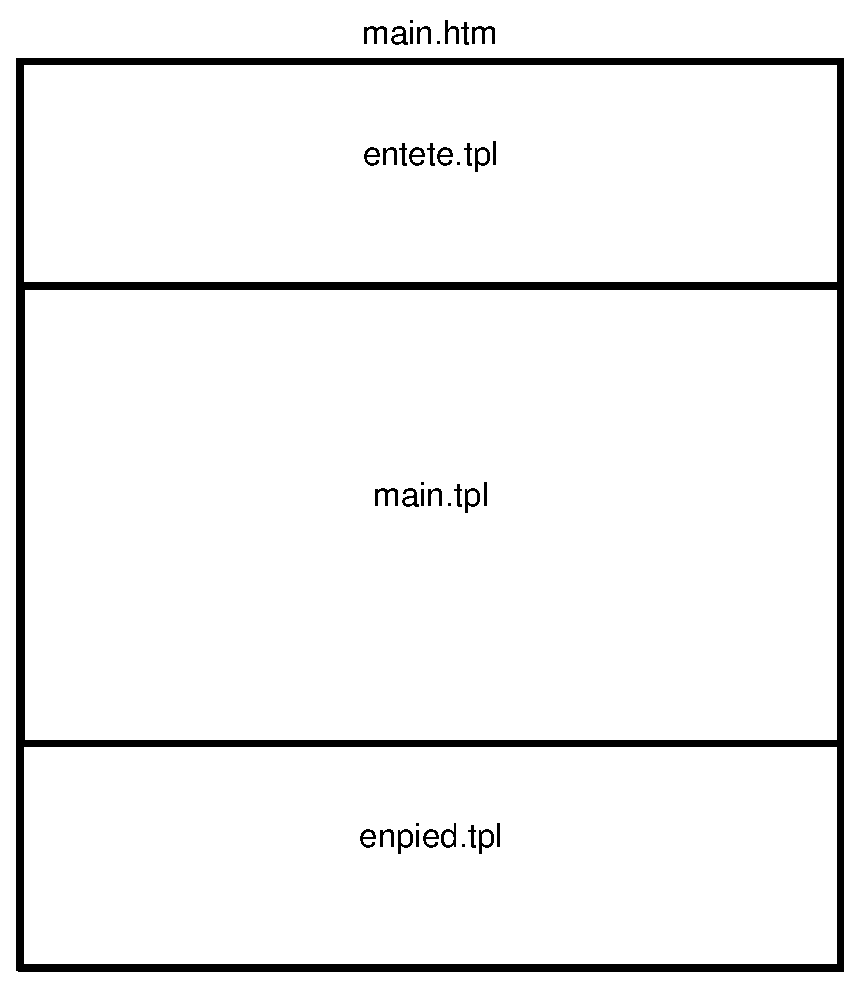
\includegraphics[width=0.7\linewidth]{dessin/templates}
\caption{}
\end{figure}

En principe, seul le modèle \textit{main.tpl} change de page en page. Il est modifié en utilisant l'assignation :
\begin{lstlisting}
$set->("nom_du_modele.tpl", "corps");
\end{lstlisting}

Un autre modèle est incorporé systématiquement : main\_js.tpl.  Il contient toutes les assignations de feuilles de style, de classes ou fonctions Javascript complémentaires utilisées dans l'application.


\subsection{Conventions de nommage}

Les templates sont stockés dans le dossier display/templates. Le dossier display/templates\_c est utilisé par Smarty pour préparer l'affichage, et doit donc être accessible en écriture au serveur web.

Pour simplfier la navigation, les templates doivent être stockés dans un sous-dossier dont le nom doit être identique au nom du sous-dossier contenant les modules PHP. Les fichiers doivent commencer par le nom du module, et se terminer par l'action correspondante, par exemple \textit{poissonList.tpl}, \textit{poissonChange.tpl}, etc. 
Cela facilite la recherche des templates en regroupant par ordre alphabétique les modèles qui portent sur le même sujet.

\section{La vue Ajax}
Nom de la classe : \textbf{VueAjaxJson}.

Elle encode le tableau fourni par la fonction \textit{set()} au format Json, et transmet la chaîne générée au navigateur, après avoir nettoyé le cache.

\section{La vue CSV}

Nom de la classe : \textbf{VueCsv}.

Fonctions disponibles : 
\begin{longtable}{|p{5cm}|p{8cm}|}
\hline
\textbf{fonction} & \textbf{Objectif} \\
\hline
\endhead
\hline\endfoot\endlastfoot
setFilename(\$filename) & indique le nom à utiliser pour générer le fichier\\

send(\$param = "") & Déclenche l'envoi du tableau vers le navigateur, au format CSV. \textit{param} peut contenir le nom du fichier souhaité. S'il est vide, le nom du fichier transmis par la fonction précédente est utilisé. Sinon, un nom de fichier, contenant la date, est généré.\\
\hline
\caption{Fonctions déclarées dans la classe VueCsv}
\end{longtable}

La fonction set() doit être utilisée pour indiquer le tableau à transformer en CSV. La classe va générer automatiquement une ligne d'entête à partir du nom des colonnes de la première ligne.

En l'état actuel, il n'est pas possible de définir des options particulières pour la génération du fichier CSV.

\section{La vue binaire}

Nom de la classe : \textbf{VueBinaire}.

Cette vue est utilisée pour envoyer des données sous forme binaire au navigateur (images, par exemple). Les données doivent avoir été auparavant générées dans un fichier du serveur web : c'est le contenu du fichier qui est transmis.

Fonctions disponibles : 
\begin{longtable}{|p{5cm}|p{8cm}|}
\hline
\textbf{fonction} & \textbf{Objectif} \\
\hline
\endhead
\hline\endfoot\endlastfoot
setParam(array \$param) & transmet un tableau contenant l'ensemble des paramètres à utiliser pour générer le fichier. Les paramètres sont les suivants : \\
& \textit{filename} : nom du fichier tel qu'il apparaîtra dans le navigateur \\
& \textit{disposition} : \textit{attachment} (fichier joint) ou \textit{inline} (affichage direct dans le navigateur) \\
& \textit{tmp\_name} : nom du fichier dans le serveur \\
& \textit{content\_type} : type mime. S'il n'est pas indiqué, le programme essaiera de le déterminer à partir du contenu du fichier \\

send() & Envoie le fichier au navigateur, en fonction des paramètres indiqués \\
\hline
\caption{Fonctions déclarées dans la classe VueBinaire}
\end{longtable}

\section{La vue PDF}

Nom de la classe : \textbf{VuePdf}.

Il s'agit d'une variante de la vue précédente. Elle accepte non pas le nom d'un fichier, mais la référence correspondant à une fonction \textit{fopen()} ou équivalente. Cette approche est nécessaire si le fichier PDF à envoyer à été stocké dans une base de données ouverte avec PDO.

Fonctions disponibles :
\begin{longtable}{|p{5cm}|p{8cm}|}
\hline
\textbf{fonction} & \textbf{Objectif} \\
\hline
\endhead
\hline\endfoot\endlastfoot
setFileReference(\$ref)& indique la référence du fichier à traiter (résultat de fopen() ou d'une lecture PDO)\\

setFilename(\$filename)& Nom du fichier tel qu'il sera transmis au navigateur. S'il n'est pas précisé, il sera généré (en cas d'attachement) \\

setDisposition(\$disp = "attachment")& Indique la manière d'envoyer le fichier au navigateur. Valeurs acceptées : \textit{attachment} ou \textit{inline}\\

send() & Envoie le fichier au navigateur, en fonction des paramètres indiqués \\
\hline
\caption{Fonctions déclarées dans la classe VuePdf}
\end{longtable}

La classe peut générer des exceptions en cas de problème.

\chapter{Génération du menu}
Pour les pages web, le menu est généré de manière dynamique :
\begin{itemize}
\item lors du premier appel à l'application ;
\item après toute opération de connexion ou de déconnexion.
\end{itemize}

Le menu est stocké en variable de session, pour accélérer l'affichage.

Il est structuré sous la forme d'une liste non ordonnée (balises \textit{ul} et \textit{li}), et contient les classes utilisées par \textit{bootstrap} pour son affichage.

\section{Fichier de description}

Le menu est généré à partir du fichier \textbf{param/menu.xml}. La branche principale s'appelle \textit{<menu>}. Voici un exemple d'entrée, qui correspond au menu d'administration :

\begin{lstlisting}
<item module="administration" label="Administration" tooltip="Administration de l'application" droits="admin">
	<item module="loginList" menulevel="1" menuorder="9" droits="admin" label="Liste des comptes locaux" tooltip="Liste des logins - identification via la base de données"/>
	<item module="appliList" droits="admin" label="ACL - droits" tooltip="applications et droits gérés"/>
	<item module="aclloginList" droits="admin" label="ACL - logins" tooltip="Logins déclarés dans le module de gestion des droits"/>
	<item module="groupList" droits="admin" label="ACL - groupes de logins" tooltip="Groupes de logins et logins rattachés aux groupes"/>
	<item module="dbparamList" droits="admin" label="Paramètres de l'application" tooltip="Liste des paramètres pérennes de l'application" />
	<item module="phpinfo" droits="admin" label="PHP info" tooltip="configuration générale du serveur PHP"/>
</item>
\end{lstlisting}

Les entrées du menu sont déclarées dans des balises \textbf{item}. Voici les attributs utilisables :

\begin{longtable}{|p{2.5cm}|c|p{9cm}|}
\hline
\textbf{Attribut} & \textbf{Requis} & \textbf{Signification} \\
\hline
\endhead
\hline\endfoot\endlastfoot
module & X & Nom du module à exécuter, tel que décrit dans le fichier actions.xml (\textit{cf.} \ref{actions} \textit{\nameref{actions}}, page \pageref{actions})\\

droits & & Droit nécessaire pour afficher l'entrée du menu. Il est possible d'indiquer plusieurs droits, en les séparant par une virgule\\

loginrequis & & Si vaut 1, l'entrée ne sera affichée que si l'utilisateur est connecté \\

onlynoconnect & & Si vaut 1, l'entrée ne sera affichée que si l'utilisateur n'est pas connecté\\

label & X & Texte affiché\\

tooltip & X & libellé affiché au survol de la souris (attribut HTML \textit{title})\\
 \hline

\caption{Liste des attributs utilisables pour décrire les entrées du menu}
\end{longtable}

Une entrée \textit{item} peut contenir d'autres entrées \textit{item}, ce qui permet de décrire les menus en cascade. Actuellement, le menu n'a été testé qu'avec 2 niveaux (menu principal horizontal, et menus verticaux associés).

L'ordre d'affichage est celui décrit dans le fichier xml.

\section{Génération en mode développement}

Si la variable \textit{APPLI\_modeDeveloppement} est positionnée à \textit{true}, le menu est généré à chaque appel.

\chapter{Gestion des langues}\label{langue}

Le framework a été conçu pour supporter plusieurs langues européennes.

Depuis juillet 2018, il utilise la fonction \textit{gettext} pour traduire tous les libellés. La mise au point a été réalisée par Alexandre Maindron, dans le cadre du projet Collec-Science \href{https://github.com/Irstea/collec}{https://github.com/Irstea/collec}.

Les fichiers de traduction sont déclarés dans le dossier locales/C/LC\_MESSAGES. Le fichier .po contient les libellés à traduire et leur traduction, le fichier .mo la valeur compilée.

Le script \textit{generate\_translation.sh} récupère tous les libellés à traduire, lance le programme \href{https://poedit.net/}{poedit}, et compile le résultat dans le fichier .mo. Le script détaille précisément les opérations effectuées, notamment la récupération des libellés dans les fichiers xml ou dans les modèles Smarty.

Les fichiers locales/fr.php et locales/en.php ne sont plus utilisés que pour définir des paramètres généraux, notamment pour traiter les formats de dates.

\chapter{Compléments sur Smarty}\label{smarty}

\section{Syntaxe générale}
Smarty est basé sur le langage PHP : il est possible d'utiliser beaucoup de mécanismes du langage, notamment les fonctions de test.

Les commandes Smarty sont encadrées dans des accolades. L'analyseur est capable de rechercher des balises dans des chaînes encadrées par des guillemets ou des cottes. Toute commande ou ordre Smarty doit toucher l'accolade ouvrante.

Les variables, comme en PHP, doivent commencer par le caractère \textit{dollar}.

\subsection{Encadrement des libellés pour gérer le multilinguisme}

Pour qu'ils puissent être pris en charge par GETTEXT et traduits dans la langue demandée, les libellés doivent être encadrés par les balises t :
\begin{lstlisting}
{t}libellé à afficher{/t}
\end{lstlisting}

\subsection{Cohabitation Javascript et Smarty}

Les fonctions Javascript sont, elles aussi, encadrées par des accolades. Pour permettre d'insérer des variables Smarty dans du code Javascript, il suffit de respecter les règles suivantes :
\begin{itemize}
\item toute commande Smarty doit impérativement toucher l'accolade ouvrante ;
\item tout code Javascript doit être séparé de l'accolade ouvrante par un espace.
\end{itemize}

Exemple :
\begin{lstlisting}
function fonctionJavascript() {
var varJavascript = {$variableSmarty};
}
\end{lstlisting}

La variable \textit{varJavascript} sera assignée avec le contenu de la variable \textit{\$variableSmarty}, transmise par Smarty.

\subsection{Affichage d'une variable}

Une variable assignée à Smarty est affichée ainsi :

Code PHP :
\begin{lstlisting}
$vue->set("contenu","varSmarty");
\end{lstlisting}

Dans le template :
\begin{lstlisting}
{$varSmarty}
\end{lstlisting}
affichera la valeur \textit{contenu}.


\subsection{Affichage d'une liste}
En général, l'interrogation de la base de données ramène un tableau associatif, chaque ligne contient un tableau avec le nom des attributs comme clé, et la valeur de l'attribut associé.

Smarty dispose d'un mécanisme permettant de traiter un tableau facilement.

Voici d'abord le code PHP :
\begin{lstlisting} 
$vue->set($instance_objetBDD->getListe(), "data");
\end{lstlisting}

Et le code permettant de l'afficher dans le template :
\begin{lstlisting}
{section name=lst loop=$data}
{$data[lst].attr1} {$data[lst].attr2}<br>
{/section}
\end{lstlisting}

Les attributs \textit{attr1} et \textit{attr2} de toutes les lignes seront affichés les uns au dessous des autres.

\subsubsection{Dans un tableau - Datatables}

Le framework utilise le composant Datatables (\url{datatables}) pour l'affichage des tableaux. Datatables a été paramétré pour trier correctement les dates (plugin qui reconnaît automatiquement les libellés de type date).

Pour qu'une table soit reconnue comme un composant Datatables, il suffit de lui rajouter la classe datatable. Voici un exemple d'utilisation :
\begin{lstlisting}
<table id="exampleList" class="table table-bordered table-hover datatable " >
<thead>
<tr>
<th>Date</th>
<th>Comments</th>
<th>status</th>
</tr>
</thead><tbody>
{section name=lst loop=$data}
<tr>
<td>
{if $droits["gestion"] == 1}
<a href="index.php?module=exampleChange&example_id={$data[lst].example_id}">
{$data[lst].example_date}
</a>
{else}
{$data[lst].example_date}
{/if}
</td>
<td>{$data[lst].comment}</td>
<td><span class="textareaDisplay">{$data[lst].example_comment}</span></td>
</tr>
{/section}
</tbody>
</table>
{/if}
\end{lstlisting}

Chaque ligne du corps est traité dans la section. Cet exemple rajoute en plus l'accès à la page de modification, selon les droits définis (\textit{cf.} \ref{droits} \textit{\nameref{droits}}, page \pageref{droits}).

Pour modifier l'ordre de tri ou d'autres paramètres du composant Datatables, le plus simple est de rajouter ce code après l'affichage du tableau :

\begin{lstlisting}
$(document).ready(function() {
	var exempleList = $("#exempleList").DataTable();
	exempleList.order([[1, 'desc'], [0, 'desc']]).draw();
});
</script>
\end{lstlisting}

L'ordre des colonnes commence à 0.

\subsubsection{Dans un select}

Dans les formulaires, des champs de type \textit{select} est souvent utilisé pour proposer une liste fermée de choix à l'utilisateur. 

Voici comment l'implémenter dans un template :

\begin{lstlisting}
<select id="container_type_id" name="container_type_id" class="form-control">
<option value="" {if $data.container_type_id == ""}selected{/if}>Selectionnez...</option>
{section name=lst loop=$container_type}
<option value="{$container_type[lst].container_type_id}" {if $container_type[lst].container_type_id == $data.container_type_id}selected{/if}>
{$container_type[lst].container_type_name}
</option>
{/section}
</select>
\end{lstlisting}

Dans cet exemple, le champ container\_container\_id doit être sélectionné à partir de la liste contenue dans \textit{container\_type}. Ici, l'utilisateur peut ne pas renseigner l'information : la première option peut être vide. Si le champ doit être obligatoire, il suffit de supprimer la première option.

Des tests sont réalisés pour positionner correctement l'indicateur \textit{selected} lors de l'affichage en modification.

\subsection{Les tests}

Les tests sont classiques, sous la forme : 
\begin{lstlisting}
{if condition_de_test}

{else}

{/if}
\end{lstlisting}

Les conditions de test sont celles de PHP, par exemple :
\begin{lstlisting}
{if strlen($variable) > 0}
...
{/if}
\end{lstlisting}

\subsection{Les variables internes}
Les sections disposent de variables permettant de connaître le nombre d'occurrences d'un tableau, l'occurrence courante... Avec des composants comme Datatables, on ne les utilise guère.

Par contre, il est parfois nécessaire de réaliser quelques calculs : il est possible d'assigner des variables facilement (le code a été simplifié par rapport aux premières versions) :

\begin{lstlisting}
{$variable = 0}
{$section name=lst loop=$data}
{$variable = $variable + $data[lst].montant}
{/section}
Montant total : {$variable}
\end{lstlisting}

\section{Affichage des libellés en fonction de la langue}

Comme nous l'avons vu précédemment (\textit{cf.} \ref{langue} \textit{\nameref{langue}}, page \pageref{langue}), les libellés sont stockés dans la variable \$LANG. Il est alors assez facile de les afficher dans le template. Voici un exemple correspondant à l'affichage du libellé \textit{Rechercher} :
\begin{lstlisting}
<button name="{$LANG[message].21}>
\end{lstlisting}


\section{Organisation des formulaires de saisie}

En raison du parti-pris du framework de séparer toutes les actions et de pouvoir leur imposer des droits différents, la gestion d'un formulaire de saisie est un peu compliquée. À partir du même formulaire, il faut pouvoir aussi bien déclencher l'écriture d'une information (\textit{write}) que supprimer l'enregistrement (\textit{delete}). 

Il est possible de gérer deux formulaires différents, l'un étant dédié uniquement au bouton \textit{Supprimer}. L'approche actuelle est plutôt d'utiliser du javascript pou générer automatiquement l'action correspondante.

Voici un exemple de formulaire implémentant ce fonctionnement :

\begin{lstlisting}
<form class="form-horizontal protoform" id="exampleForm" method="post" action="index.php">
<input type="hidden" name="example_id" value="{$data.example_id}">
<input type="hidden" name="moduleBase" value="example">
<input type="hidden" name="action" value="Write">

<div class="form-group center">
      <button type="submit" class="btn btn-primary button-valid">{$LANG["message"].19}</button>
      {if $data.example_id > 0 }
      <button class="btn btn-danger button-delete">{$LANG["message"].20}</button>
      {/if}
 </div>
</form>
\end{lstlisting}

Le formulaire doit comprendre la classe \textit{protoform}, et deux champs cachés : \textit{moduleBase} et \textit{action}. Les boutons doivent être des classes \textit{button-valid} ou \textit{button-delete}, pour respectivement déclencher l'écriture ou la suppression de l'enregistrement.

Le code Javascript associé (déjà déclaré dans le framework) va permettre de modifier le contenu du champ \textit{action} si le bouton \textit{Supprimer} est actionné. Le contrôleur reconstituera le module demandé en associant les deux champs.